\sectionbreak \section{ \standartTitleFont
  Модуль DataManipulator
}

\subsection{ \standartTitleFont
  Назначение и описание модуля DataManipulator
} 

{\standartFont

  \par Модуль DataManipulator предназначен для различного рода обработки данных, с целью получения наборов данных необходимых для обучения моделей неройнных сетей. 
  
  \par
}

\subsection{ \standartTitleFont
  Главное меню модуля DataManipulator. 
} 

{\standartFont

  \par В главном меню модуля DataManipulator представлены основные направления для обработки данных. Предоставляется выбор, с каким форматом данных будет происходить работа: с OCDF- или TDF-форматом. В главном меню также можно выбрать пункт, позволяющий создать TDF-данные на основе OCDF-данных. Также имеется пункт, который выводит на экран краткую информацию о форматах данных и о самом модуле DataManipulator. Внешний вид меню можно увидеть на рисунке \ref{fig:mainMenu}
 
  \par

  \begin{figure}[H]
    \centering
    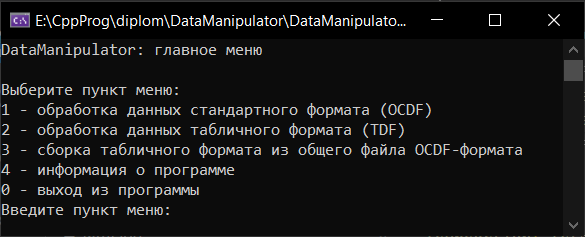
\includegraphics{images/mainMenu.png}
    \caption{главное меню модуля DataManipulator} 
    \label{fig:mainMenu}
  \end{figure}

}

\subsection{ \standartTitleFont
  Меню обработки данных OCDF-формата модуля DataManipulator. 
} 

\subsubsection{ \standartTitleFont
  Считывание OCDF-данных из файла. 
} 

{\standartFont

  \par Для того, чтобы попасть в меню по обработке данных OCDF-формата будет предложено для начала их загрузить из файла. Это показано на рисунке на рисунке \ref{fig:readOCDFst1}

  \begin{figure}[H]
    \centering
    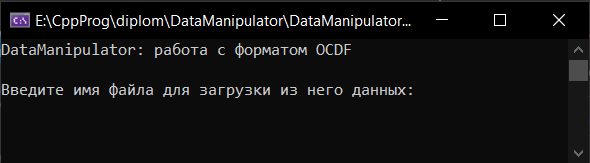
\includegraphics[width=\textwidth]{images/readOCDFstage1.png}
    \caption{указание файла для загрузки из него OCDF-данных.} 
    \label{fig:readOCDFst1}
  \end{figure}

  \par Вводим путь к файлу или перетаскиваем файл в консоль для получения его абсолютного пути и нажимаем Enter. После этого будет предложено ввести количество данных, которые необходимо считать из файла. Это показано на рисунке \ref{fig:readOCDFst2}

  \begin{figure}[H]
    \centering
    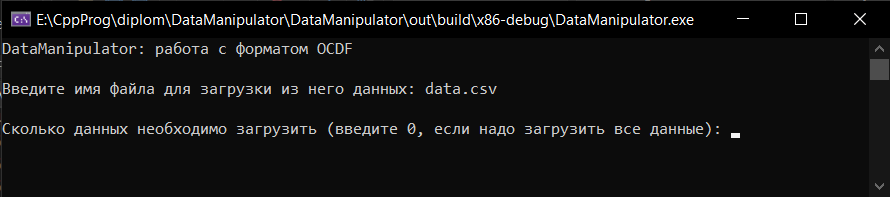
\includegraphics[width=\textwidth]{images/readOCDFstage2.png}
    \caption{указание необходимого количества данных для считывания.} 
    \label{fig:readOCDFst2}
  \end{figure}

  \par Есть несколько особенностей, при вводе количества данных. В случае, если будет введён 0 или число, превышающее количество данных в файле, то будут считаны все данные, которые есть в файле. Если будет введено отрицательное число или хотя бы один симвлом, отличный от цифр, то программа выдаст предупреждение о некорректном вводе данных, показанное на рисунке \ref{fig:readOCDFerror1}, и предложит ввести путь к файлу и необходимое количество данных для считывания снова. 

  \begin{figure}[H]
    \centering
    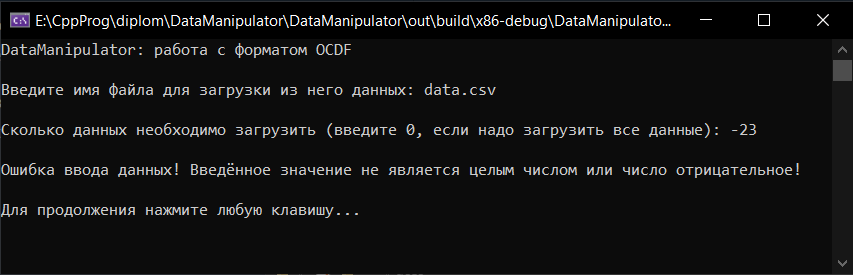
\includegraphics[width=\textwidth]{images/readOCDFerror1.png}
    \caption{предупреждение об ошибке при вводе необходимого количества данных для считывания.} 
    \label{fig:readOCDFerror1}
  \end{figure}

  \par Могут возникнуть и другие предупреждения, связанные непосредственно с самим файлом. Если файл с данными не существует, или этот файл пуст, или данные в нём не представленны в необходимом формате, то возникнет предупреждение о невозможности чтения данных, представленное на рисунке \ref{fig:readOCDFerror2}

  \begin{figure}[H]
    \centering
    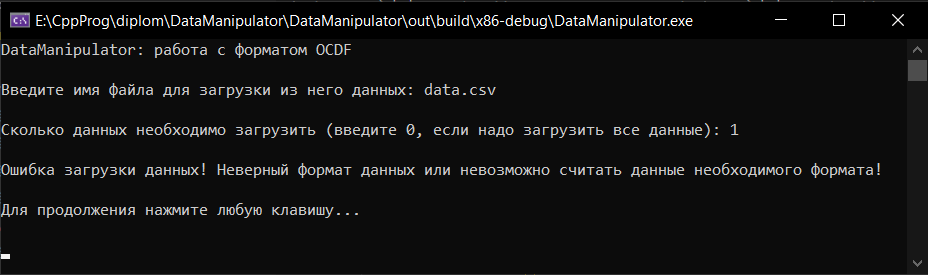
\includegraphics[width=\textwidth]{images/readOCDFerror2.png}
    \caption{предупреждение об ошибке чтения данных.} 
    \label{fig:readOCDFerror2}
  \end{figure}

  \par Как уже понятно, чтение данных происходит в текстовом режиме. Однако существует возможность считывать данные, которые представлены в бинарном виде. Для этого необходимо, чтобы файл имел расширение .bin, иначе чтение данных будет происходить в текстовом режиме. Пример файла с данными в бинарном виде можно увидеть на рисунке \ref{fig:readOCDFbin}.

  \begin{figure}[H]
    \centering
    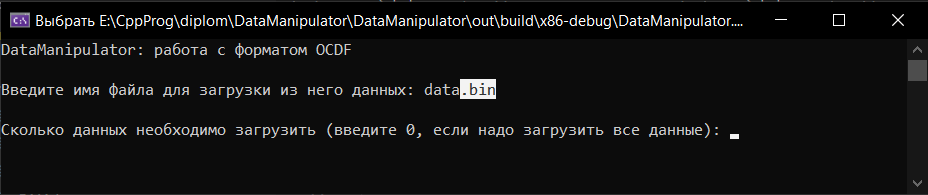
\includegraphics[width=\textwidth]{images/readOCDFbin.png}
    \caption{ввод файла с данными в бинарном виде.} 
    \label{fig:readOCDFbin}
  \end{figure}

  \par После указание файла с данными в бинарном виде будет предложено ввести количество данных, которое необходимо считать из файла. Все предупреждения, которые связаны с чтением данных и ввода значений уже разобраны выше. 

  \par
}

\subsubsection{ \standartTitleFont
  Возможности по обработке OCDF-данных. 
} 

{\standartFont

  \par После считывания OCDF-данных из файла открывается меню для работы с данными, представленное на рисунке \ref{fig:OCDFmenu}.

  \begin{figure}[H]
    \centering
    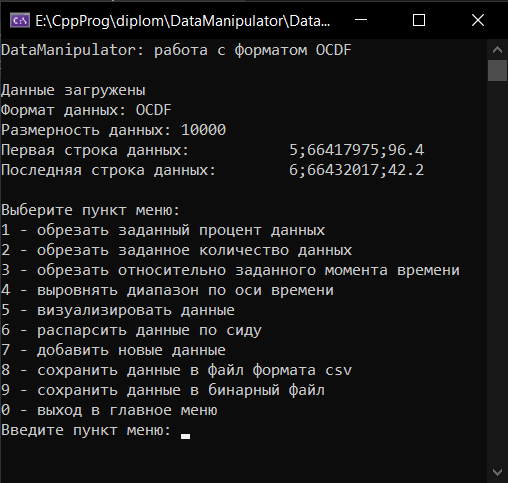
\includegraphics{images/OCDFmenu.png}
    \caption{ввод файла с данными в бинарном виде.} 
    \label{fig:OCDFmenu}
  \end{figure}

  \par В появившемся меню будет указана информация о считанных данных: формат данных, их количество, а также первая и последняя строки последовательности данных. После идёт выбор действий, которые можно совешить над данными. Каждое из них подробно будет разобрано ниже.

  \par
}

\subsection{ \standartTitleFont
  Обезка OCDF-данных. 
} 

\subsubsection{ \standartTitleFont
  Обрезка OCDF-данных по заданному проценту. 
} 

{\standartFont
  
\begin{figure}[H]
  \centering
  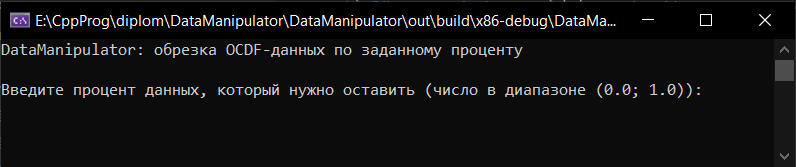
\includegraphics{images/OCDFcutpercentstage1.png}
  \caption{ввод процента для обрезки данных.} 
  \label{fig:OCDFcutper1}
\end{figure}

}

\subsubsection{ \standartTitleFont
  Обрезка OCDF-данных по заданному количеству. 
} 

\subsubsection{ \standartTitleFont
  Обрезка OCDF-данных по заданному моменту времени. 
} 